\documentclass{standalone}
\usepackage{tikz}
\tikzset{block/.style = {draw, fill=white, very thick, rectangle, minimum height=1cm, minimum width=2cm},}
\begin{document}
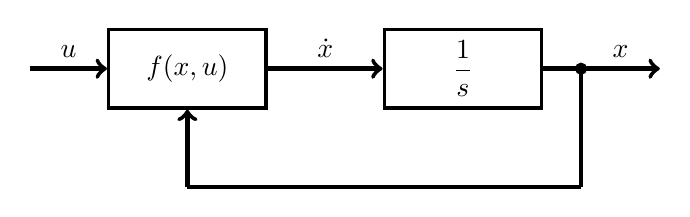
\begin{tikzpicture}[scale=2]
    \coordinate(sum)at(-1,0){};
    \node[block, right of=sum, node distance=2cm](c){$f(x,u)$};
    \draw[->,ultra thick](-1,0)--(c.180)node[midway, above]{$u$};

    %\draw[->,ultra thick](sum.0)--(c.180);
    \filldraw[black](2.5,0)circle(1pt);

    \draw[->,ultra thick](2.5,0)--(3,0)node[midway, above]{$x$};
    \draw[-,ultra thick](2.5,-0.75)--(2.5,0);

    %\node[block]at(0.75,-0.75)(h){$H(s)$};
    \node[block]at(1.75,0)(p){$\displaystyle\frac{1}{s}$};

    \draw[-,ultra thick](p.0)--(2.5,0);
    \draw[->,ultra thick](c.0)--(p.180)node[midway, above]{$\dot x$};

    %\draw[->,ultra thick](2.5,-0.75)--(h.0);
    %\draw[-,ultra thick](h.180)--(-1,-0.75);
    \draw[-,ultra thick](2.5,-0.75)--(0,-0.75);
    \draw[->,ultra thick](0,-0.75)--(c.270);
\end{tikzpicture}
\end{document}